\newpage

\subsection{Spilbeskrivelse}

PC = Player Character
RNG = Random Number Generator

Spillet designes som et text-based spil, hvilket er en spilgenre hvor brugeren interagerer med spillet igennem tekst beskrivelser. Spillet består overordnet af fire dele med hver deres ansvar: en grafisk brugergrænseflade, en database, en back-end til netværkskommunikation, samt selve spil logikken. Brugergrænsefladen gør det muligt for brugeren at integrere med spillet. Den vil bestå af en række forskellige vinduer med hver sit formål (login screen, gameplay screen og settings screen), der hovedsageligt vil indeholde knapper og beskrivende tekst. Databasens ansvar er at gemme de enkelte spil. Databasen er en relationel database som sammenholder de enkelte brugeres profiler (Username og password) med informationer omkring deres fremskridt i spillet, såsom placering, items og stats. Det skal være muligt for en bruger at hente sine gemte spil ned på flere forskellige enheder. Til dette skal der bruges en netværksforbindelse til databasen.   

\subsection{Login-screen}
Det første brugeren bliver mødt af er en login-skærm. Her skal brugeren enten indtaste sine login-oplysninger eller oprette sig en profil i systemet. Systemet har en database hvor alle profiler er lagret. Herunder ses en illustration af spillets login-screen. 

\begin{figure}[H]
\centering
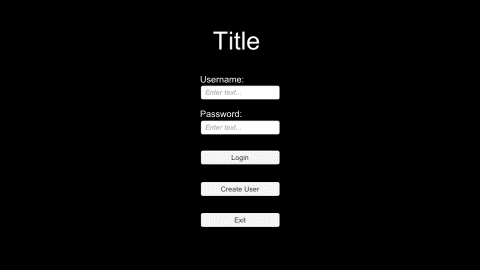
\includegraphics[width = \textwidth]{02-Body/Images/Loginscreen-udkast.png}
\caption{ssss}
\label{fig:Loginscreen-udkast}
\end{figure}

\subsection{Core gameplay layout}
PC kommer ind i et rum (se billede 2).  Brugeren bliver præsenteret med en beskrivelse af rummet, en liste af elementer i rummet, og en række muligheder for at interagere med rummet (interaktionen foregår ved at trykke på knapperne markeret “Button” i billede 2). Når brugeren er færdig med at interagere med rummet, forlader de det ved at vælge en retning (“go north/south/east/west”). 
Dette fører dem ind i et nyt rum, mappet opdateres og loopet starter forfra.
Bevægelsen i spillet kan gøres i de forklarede fire retninger. Disse retninger indikerer for spilleren hvilke rum de kan bevæge sig ind i relativt til det rum de er i, der kunne f.eks. være rum, som kun har en vej ind og en vej ud, så kan man ikke gå andre veje end vejen man kom ind. North/south/east og west retningerne er baseret på et kompas, så derfor ville North resultere i at bevæge spillerens karakter opad, South nedad osv.
Rum på mappet loades efterhånden som man besøger dem.

\begin{figure}[H]
\centering
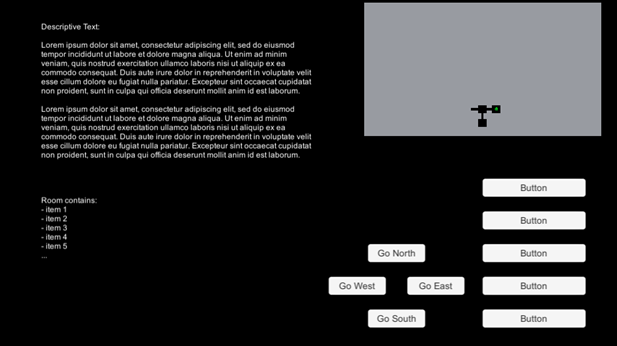
\includegraphics[width = \textwidth]{02-Body/Images/SpilLayout-udkast.png}
\caption{sss}
\label{fig:Spillayout-udkast}
\end{figure}

\begin{figure}[H]
\centering
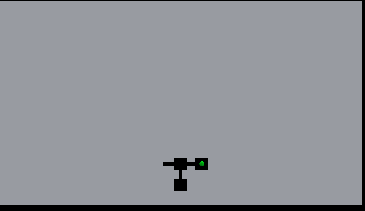
\includegraphics[width = \textwidth]{02-Body/Images/Map-closeup.png}
\caption{Closeup Screenshot af mappet}
\label{fig:Spillayout-udkast}
\end{figure}

Et rum kan indeholde fjender, som skal bekæmpes før man kan tilgå resten af rummet. Kamp foregår ved at spillet “slår en terning“ (RNG) for både PC og fjenden og lægger deres “combat stat” til slaget. Den som slår højest giver en vis mængde skade til modstanderen, afhængigt af deres “damage stat”. Denne skade trækkes fra karakterens liv. Når en karakters liv bliver mindre eller lig 0 dør karakteren. Hvis spiller karakteren dør taber brugeren spillet.  Hvis hverken PC eller fjenden er død efter en kamp får brugeren valget mellem at flygte (gå tilbage til det rum de kom fra) eller fortsætte kampen (start loopet forfra). 
Det er muligt at finde våben og udrustning i banen, som kan bruges til at forbedre karakterens stats. 

\begin{figure}[H]
\centering
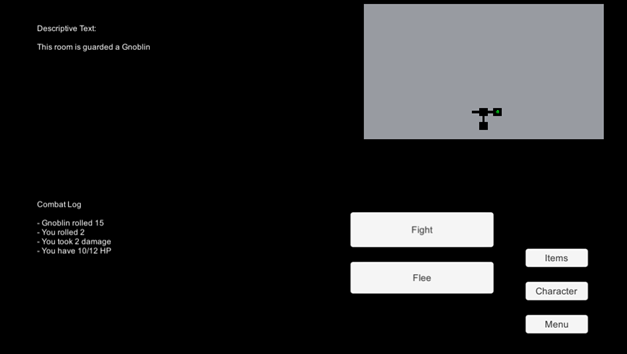
\includegraphics[width = \textwidth]{02-Body/Images/CombatScreen-udkast.png}
\caption{}
\label{fig:Combat-udkast}
\end{figure}

\subsection{Settings}
Det skal være muligt for spilleren at tilgå en menu med spillets indstillinger. Her skal det være muligt for brugeren at tilpasse spillets layout indstillinger så som resolution og window size. Det skal ligeledes være muligt at justere lydstyrken for spillet. En illustration af hvordan denne menu kunne se ud er vist på figur x.

\begin{figure}[H]
\centering
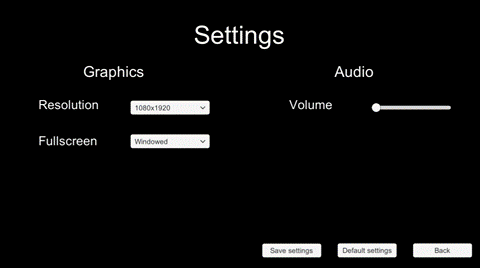
\includegraphics[width = \textwidth]{02-Body/Images/SettingsMenu-udkast.png}
\caption{Screenshot af settings menuen}
\label{fig:Settings-udkast}
\end{figure}
